\chapter{Introduction \`a Moodle et \`a son architecture modulaire}
Moodle est un environnement d'apprentissage en ligne (LMS, \textit{Learning Management System}) cr\'e\'e par Martin Dougiamas\footnote{\url{https://docs.moodle.org/35/en/History}}.
Cette plateforme est un logiciel libre d\'evelopp\'e en \texttt{PHP} sous licence GPL (\textit{GNU Public License})\footnote{\url{http://docs.moodle.org/dev/License}} dont le code source se trouve sur GitHub\footnote{\url{https://github.com/moodle/moodle}}.

Moodle est un outil modulaire o\`u chaque enseignant peut cr\'eer ses cours comme il le souhaite.
Chaque cours est d\'ecompos\'e en sections d\'efinies en semaines, modules, th\`emes ou selon diverses autres configurations.
Chaque section comporte plusieurs activit\'es: un texte \`a lire, des documents \`a t\'el\'echarger, un forum pour \'echanger, un sondage ou questionnaire en ligne \`a compl\'eter, un devoir \`a remettre, et plus encore.
Chaque activit\'e est hautement configurable.
Par exemple, un devoir peut \^etre fait individuellement ou en \'equipe, avoir une date et une heure de d\'ebut et de fin de disponibilit\'e avec un d\'elai de retard permis, etc.
Dans les questionnaires en ligne, un enseignant peut cr\'eer une banque de questions et s\'electionner les questions d\'esir\'ees ou laisser le syst\`eme choisir les questions al\'eatoirement.

\section{Activit\'e <<Questionnaire>>}
Ce projet s'attarde \`a l'activit\'e <<Questionnaire>> de Moodle, plus sp\'ecifiquement sur la question de type <<Texte long>> (parfois appel\'e <<Composition>>, selon la version de Moodle).
Tout d'abord, qu'est-ce qu'une activit\'e <<Questionnaire>>?
Une telle activit\'e permet \`a l'enseignant de cr\'eer un formulaire en ligne auquel les \'etudiants devront r\'epondre.
Il peut s'agir, par exemple, d'une \'evaluation sommative qui sera cumul\'ee au carnet de notes Moodle, d'une \'evaluation formative ou d'un atelier qui pourra \^etre fait plusieurs fois jusqu'\`a ce que l'\'etudiant atteigne une note pr\'ed\'efinie.
Parmi les options les plus utiles de cette activit\'e, on retrouve (toutes optionnelles): d\'ebut et fin de disponibilit\'e du questionnaire, temps disponible \`a partir de l'ouverture du questionnaire, note de passage, ordre al\'eatoire des questions, nombre de tentatives possibles, etc.

Chaque questionnaire est compos\'e d'un nombre de questions choisies dans une banque de questions.
Les questions peuvent avoir un ordre pr\'ecis ou \^etre choisies al\'eatoirement parmi un ensemble de questions.
Voici une liste non exhaustive des types de questions:
\begin{description}
  \item[Choix multiple]
  
  Affiche une liste de boutons radio ou de cases \`a cocher;
  
  \item[R\'eponse courte]
  
  Affiche un champ texte pouvant accueillir quelques mots;
  
  \item[Num\'erique]
  
  Affiche un champ texte pour valeur num\'erique pouvant prendre en compte une unit\'e de mesure (par exemple, km, cm ou m);
  
  \item[Question Cloze]
  
  Permet de cr\'eer un texte lacunaire, chaque \og trou \fg{} pouvant \^etre rempli avec une sous-question de type <<~choix multiples~>>, r\'eponse courte ou num\'erique;
  
  \item[Composition]
  
  Affiche un champ texte multilignes, multilignes avec police monospace ou \textit{WYSIWYG (What You See Is What You Get)}, dans lequel
  l'\'etudiant doit \'ecrire un texte \`a d\'eveloppement.
\end{description}
Toutes les questions, sauf celles de type <<Composition>>, peuvent se corriger automatiquement \`a un moment d\'ecid\'e par l'enseignant.
La correction peut se faire \`a la saisie de la r\'eponse pour une r\'etroaction en direct ou apr\`es la soumission du questionnaire.
Par exemple, dans un examen \`a choix de r\'eponses, les \'etudiants pourraient voir leur note d\`es qu'ils ont termin\'e leur examen.

\medskip

\begin{minipage}{\linewidth}
Chaque type de question se corrige de mani\`ere diff\'erente:
\begin{description}
  \item[Choix multiple]
  
  Chaque bouton radio ou case \`a cocher vaut un certain nombre de points, allant de $-100~\%$ \`a $+100~\%$ de la valeur de la question.
  Par exemple, dans une question valant 2 points avec plusieurs choix possibles, chacune des deux bonnes r\'eponses pourrait ajouter 1 point et chacune des mauvaises r\'eponses pourrait enl\`ever 1 point.
  Dans un tel cas, l'\'etudiant pourrait donc avoir une note n\'egative;
  
  \item[R\'eponse courte]
  
  L'enseignant peut sp\'ecifier plusieurs mots ou expressions r\'eguli\`eres qui valent un certain nombre de points. Par exemple,
  \`a la question \og{} En quelle ann\'ee Christophe Colomb a-t-il d\'ecouvert l'Am\'erique? \fg{}, une r\'eponse contenant \og 1492 \fg{} pourrait donner tous les points alors qu'une r\'eponse correspondant \`a l'expression r\'eguli\`ere \og 15(.*)si\`ecle \fg{} pourrait donner la moiti\'e des points;
  
  \item[Num\'erique]
  
  L'enseignant peut sp\'ecifier plusieurs bonnes r\'eponses en tenant compte de diverses unit\'es de mesure.
  Par exemple, les r\'eponses \og 2 km \fg{} et  \og~2000~m~\fg{} pourraient \^etre accept\'ees;
  
  \item[Question Cloze]
  
  Chaque \og trou \fg{} du texte lacunaire est corrig\'e selon le type de question utilis\'e dans ce \og trou \fg{}.
  Si on utilise une question de type R\'eponse courte dans un \og trou \fg{}, Moodle utilisera la correction correspondant \`a ce type de question.
  
  \item[Composition]
  
  Moodle ne corrige pas automatiquement ce type de question.
  L'enseignant ou le correcteur doit donc corriger manuellement chaque copie.
\end{description}
\end{minipage}

\section{Question de type <<Composition>>}

\begin{figure}[htbp]
  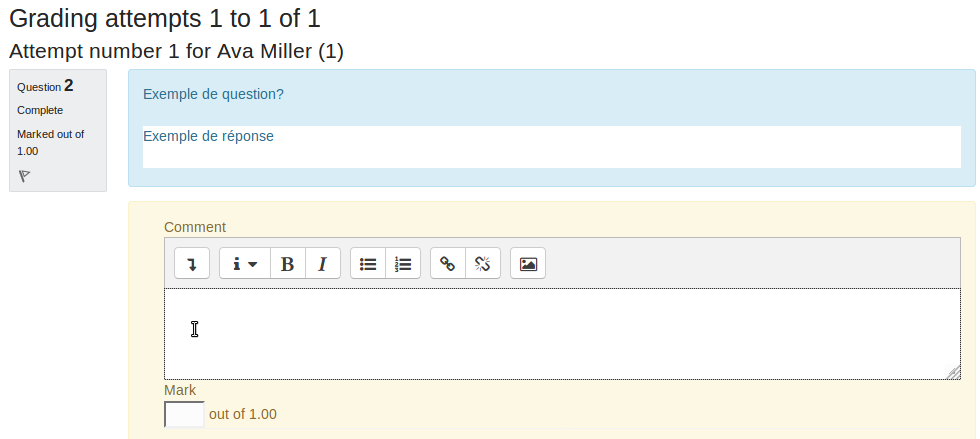
\includegraphics[scale=0.55]{images/correction-manuelle.png}
  \caption{Interface du module de correction manuelle de Moodle.}
  \label{correction-manuelle}
\end{figure}

D\`u \`a sa nature, le type de question <<Composition>> est le seul qui ne peut pas se corriger automatiquement par Moodle.
L'enseignant doit donc corriger manuellement toutes les r\'eponses \`a l'aide du module de correction manuelle, tel qu'illustr\'e \`a la figure~\ref{correction-manuelle}.
L'enseignant peut choisir de corriger le questionnaire en entier, un \'etudiant apr\`es l'autre.
Il peut aussi choisir de corriger une question \`a la fois, affichant ainsi les r\'eponses de tous les \'etudiants \`a cette question sur une seule page.
Cette derni\`ere m\'ethode est appr\'eci\'ee de plusieurs enseignants, car elle permet de comparer toutes les r\'eponses donn\'ees et ainsi corriger de mani\`ere plus uniforme.

Notre projet consiste \`a faciliter le travail du correcteur en cr\'eant un nouveau module Moodle qui\ldots
\begin{enumerate}
  \item Affichera la r\'eponse de l'\'etudiant et la r\'eponse de l'enseignant c\^ote \`a c\^ote afin de faciliter la t\^ache au correcteur;
  \item Utilisera la racination ou la lemmatisation afin de mieux identifier les mots-cl\'es, peu importe leur accord;
  \item Surlignera les mots-cl\'es, fournis par l'enseignant, tant dans la r\'eponse de l'\'etudiant que celle de l'enseignant.
\end{enumerate}
Le module d'extension propos\'e sera utile pour les questions \`a d\'eveloppement pour les textes descriptifs, et aussi pour des segments de code (en programmation), mais le sera moins pour les textes d'opinion o\`u il n'y a pas de \og bonne \fg{} r\'eponse.

\section{Les modules d'extension Moodle}
L'aspect modulaire de Moodle est visible tant pour les enseignants que pour les programmeurs.
Presque toutes les fonctionnalit\'es de Moodle sont configur\'ees \`a l'aide de modules d'extension.
Il y a des modules d'extension pour changer l'apparence du site, pour exporter les donn\'ees, pour changer le fonctionnement des questions, etc.
Chaque module d'extension est d\'evelopp\'e par un membre de la communaut\'e.
La plupart de ces modules d'extension se retrouvent sur GitHub et quelques-uns se retrouvent dans le r\'epertoire des module d'extension Moodle\footnote{\url{https://moodle.org/plugins/}}.
Pour ajouter un nouveau module d'extension \`a ce r\'epertoire, il faut qu'il soit approuv\'e par un comit\'e Moodle.
Le processus d'approbation est pr\'esent\'e \`a la figure~\ref{plugin-workflow}.
%
Il est aussi possible d'installer un module d'extension non officiel en installant les fichiers au bon endroit dans l'arborescence Moodle.
\begin{figure}[h!]
  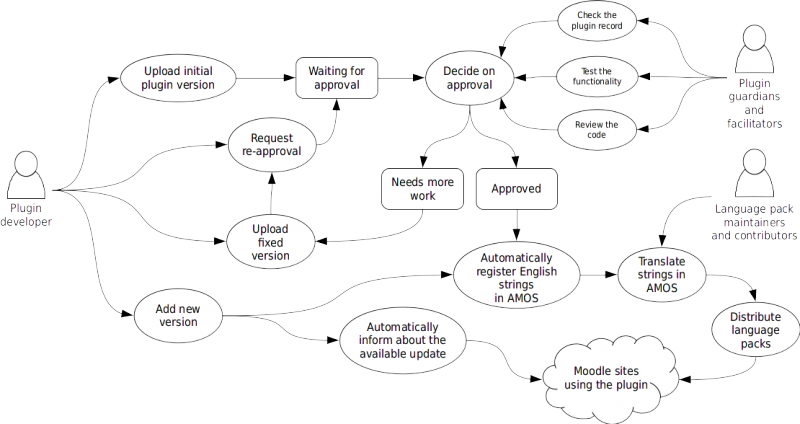
\includegraphics[scale=0.7]{images/plugin-contribution-workflow.png}
  \caption[Flux d'acception d'un module d'extension Moodle]{Flux d'acception d'un module d'extension Moodle (\href{https://docs.moodle.org/dev/Plugin_contribution}{\url{https://docs.moodle.org/dev/Plugin\_contribution}}).}
  \label{plugin-workflow}
\end{figure}

Pour ajouter des fonctionnalit\'es \`a l'activit\'e questionnaires, il y a trois types de modules d'extension \`a consid\'erer: un rapport de questionnaire, un type de question et un comportement de question.

\subsection{Module d'extension <<Rapport de questionnaire>> (\textit{Quiz report})}
Un rapport de questionnaire sert principalement \`a corriger les r\'eponses des \'etudiants.
On peut aussi se servir de ce type de module d'extension pour afficher les r\'eponses et les notes des \'etudiants pour un questionnaire sous forme de rapport.
Finalement, on peut aussi s'en servir afin de modifier les champs disponibles dans la configuration de base d'un questionnaire.
Lors de l'analyse initiale du projet, il avait \'et\'e pr\'evu de se servir uniquement de ce type de module d'extension, car nous voulions uniquement modifier l'interface de correction.
Par contre, comme nous voulions ajouter une liste de mots-cl\'es \`a une question et que ce type de module d'extension permet de modifier seulement le questionnaire, d\'evelopper uniquement un module d'extension de ce type n'\'etait pas suffisant.

\subsection{Module d'extension <<Type de question>> (\textit{Question type})}
Chaque question est d\'efinie par un type de question (voir la liste \`a la section~1.1).
Un nouveau type de question ajoute donc plus de choix \`a l'enseignant d\'esirant cr\'eer un questionnaire.
Chaque type de question poss\`ede des champs personnalis\'es et change l'apparence de la question pour l'\'etudiant et l'enseignant.

Nous ne voulions pas modifier le module d'extension \og Type de question Composition \fg{} car les nouvelles fonctionnalit\'es ne seront pas utiles pour tous les types de texte: un texte d'opinion pour un cours de philosophie, par exemple, n'aura pas n\'ecessairement besoin d'une liste de mots-cl\'es et d'une fonctionnalit\'e de comparaison de textes.
La possibilit\'e de cr\'eer un module d'extension qui ajoute un nouveau type de question qui \'etend les fonctionnalit\'es du \og Type de question Composition \fg{} par h\'eritage a \'et\'e analys\'ee, mais il semble que ce n'est pas possible avec Moodle.
Seule alternative restante: se baser sur le \og Type de question Composition \fg{} pour cr\'eer un tout nouveau module d'extension.
Ce nouveau module d'extension utilise les m\^emes fonctionnalit\'es que le \og Type de question Composition \fg{}, mais en enlevant quelques fonctionnalit\'es (remise de pi\`ece jointe et \'ecriture dans un \textit{WYSIWIG}) et en ajoutant quelques autres (mots-cl\'es et r\'eponse de l'enseignant).

\subsection{Module d'extension <<Comportement de question>> (\textit{Question behaviour})}
Un comportement de question permet les op\'erations suivantes:
\begin{enumerate}
  \item Ajouter du code \`a la suite de la question, par exemple, un bouton \og V\'erifier \fg{} ou une zone de texte commentaire;
  
  \item Modifier la m\'ethode de correction, par exemple, une correction manuelle, une correction automatique instantan\'ee quand l'\'etudiant r\'epond ou une correction automatique lorsque le test est termin\'e;
  
  \item Modifier l'affichage des questions, par exemple, afficher une question suppl\'ementaire si l'\'etudiant a plusieurs fautes ou donner des indices \`a l'\'etudiant sous r\'eserve d'une perte de points.
\end{enumerate}
Comme nous d\'esirons une correction manuelle, nous pouvons utiliser le comportement \texttt{ManualGraded}.
De plus, comme il est possible de contr\^oler directement l'apparence de la r\'eponse et de la question avec un module d'extension <<Type de question>>, il n'est pas n\'ecessaire de cr\'eer un module d'extension \og Comportement de question \fg{}.

\section{Choix du module d'extension \`a cr\'eer}
Un module d'extension <<Type de question>> est obligatoire dans ce projet afin d'ajouter les champs mots-cl\'es et r\'eponse de l'enseignant.
Nous n'avons pas besoin des fonctionnalit\'es qu'offre le module d'extension <<Comportement de question.>>
Il reste \`a d\'eterminer s'il faut utiliser un module d'extension <<Rapport de questionnaire>> ou non.
En analysant le code du module d'extension de correction manuelle fourni de base avec Moodle (\texttt{quiz\_grading}), on d\'ecouvre que ce module fournit l'interface de correction, mais que la r\'eponse de chaque \'etudiant est g\'er\'ee par le type de question dans un affichage en lecture seulement.
Les fonctionnalit\'es pr\'evues peuvent donc se trouver autant dans le type de question que dans un rapport de questionnaire, la complexit\'e du code est la m\^eme pour les deux cas.
Puisqu'il doit y avoir obligatoirement un module d'extension <<Type de question>> et qu'un nouveau module d'extension <<Rapport de questionnaire>> est facultatif, nous avons d\'ecid\'e de ne faire qu'un seul module d'extension.
En outre, le fait d'avoir un seul module d'extension facilite grandement l'installation pour d'autres administrateurs Moodle.
